\documentclass[preview]{standalone}

\usepackage{amsmath}
\usepackage{amssymb}
\usepackage{stellar}
\usepackage{bettelini}

\hypersetup{
    colorlinks=true,
    linkcolor=black,
    urlcolor=blue,
    pdftitle={Biologia},
    pdfpagemode=FullScreen,
}

\begin{document}

\title{Biologia}
\id{biologia-occhio}
\genpage

\plain{Gli occhi trasformano lo stimolo delle lunghezze d'onda della luce in segnali elettrici.
Questo processo si chiama trasfuzione sensoriale.}

\begin{snippet}{eye-illustration}
    \begin{center}
    \begin{figure}[ht]
        \centering
        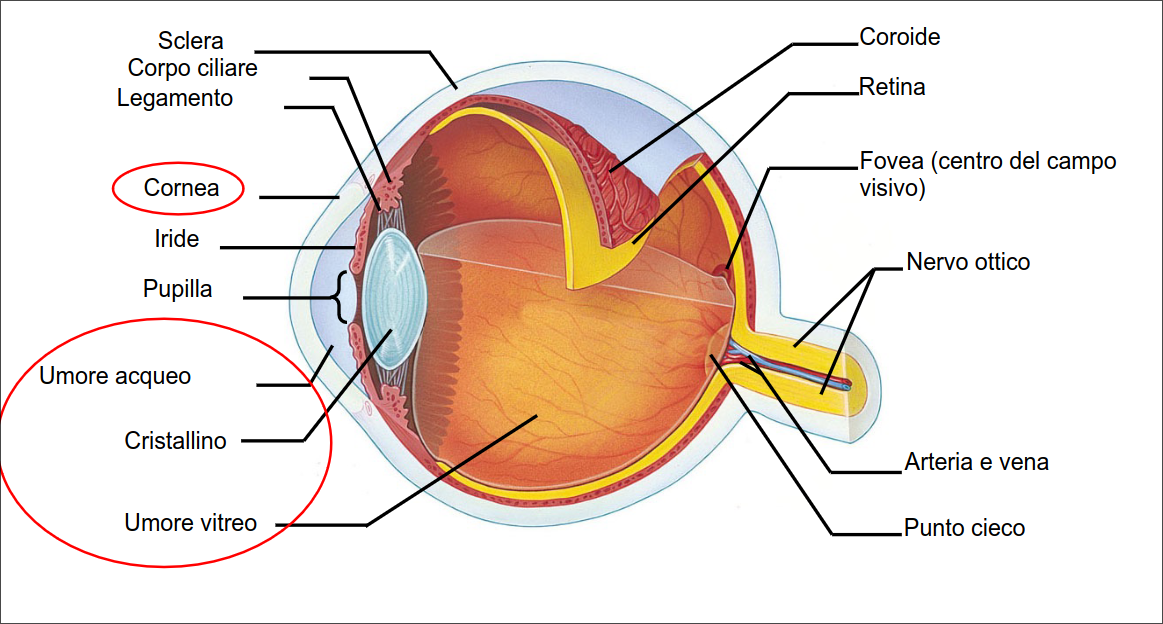
\includegraphics[width=0.9\textwidth]{./resources/eye.png}
    \end{figure}
    \end{center}
\end{snippet}

\plain{Il nervo ottico trasporta gli impulsi elettrici verso il cervello.}

\begin{snippetdefinition}{sclera-definition}{Sclera}
    La \textit{sclera} costituisce la parte bianca protettiva dell'occhio.
\end{snippetdefinition}

\begin{snippetdefinition}{retina-definition}{retina}
    La \textit{retina} è l'ultimo strato interno dell'occhio, dove la entra la luce.
    In questa zona vi sono i fotorecettori (recettori sensoriali) che captano lo sttimolo (lunghezza d'onda).
\end{snippetdefinition}

\begin{snippetdefinition}{coroide-definition}{Coroide}
    Strato pigmentato circondato dalla sclera. È estremamente vascolarizzato, quindi rifornisce
    di nutrienti e ossigeno quasi tutte le cellule dell'occhio.
\end{snippetdefinition}

\begin{snippetdefinition}{umore-vitreo-definition}{Umore vitreo}
    Sostanza gelatinosa che contribuisce a mantenere la forma del bulbo oculare e fissa la
    retina sulla coroide.
\end{snippetdefinition}

\begin{snippetdefinition}{umor-acqueo-definition}{Umor acqueo}
    Sostanza meno viscosa dell'umore vitreo secreta dalle cellule del corpo ciliare. Contribuisce
    a mantenere la forma del bulbo oculare. Fornisce nutrimento e ossigeno al cristallino,
    all'iride e alla cornea e rimuove le sostanze di rifiuto
\end{snippetdefinition}

\begin{snippetdefinition}{cornea-definition}{Cornea}
    La \textit{cornea} è una lenta che possiede una curva per deviare la luca, e farla atterrare in un punto preciso.
\end{snippetdefinition}

\begin{snippetdefinition}{fovea-definition}{Fovea}
    Punto della retina corrispondente al centro del campo visivo, in cui sono altamente
    concentrati i fotorecettori.
\end{snippetdefinition}

\begin{snippetdefinition}{pupilla-definition}{Pupilla}
    La \textit{pupilla} è una fessura attraverso la quale penetra la luce. 
\end{snippetdefinition}

\begin{snippetdefinition}{cristallino-definition}{Cristallino}
    Lente che mette a fuoco la luce sulla retina, mantenuto in posizione da appositi legamenti.
\end{snippetdefinition}

\begin{snippetdefinition}{punto-cieco-definition}{Punto cieco}
    Punto della retina in cui non ci sono fotorecettori; dunque, la luce messa a fuoco sul punto
    cieco non è rilevabile.
\end{snippetdefinition}

\begin{snippetdefinition}{iride-definition}{Iride}
    L'\textit{iride} è un muscolo con due funzioni
    \begin{itemize}
        \item regolazione del diametro della pupilla;
        \item blocco della quantità di luce in eccesso.
    \end{itemize}
\end{snippetdefinition}

\section{Accomodamento del cristallino}

\begin{snippet}{accomodamento-cristallino}
    La forma del cristallino è controllata da muscoli ciliari, attaccati alla coroide e ai legamenti
che tengono sospeso il cristallino. Quando l'occhio mette a fuoco un oggetto da vicino,
questi muscoli si contraggono e tirano la coroide verso il cristallino, riducendo la tensione
sui legamenti. In tali condizioni, il cristallino elastico diventa più spesso e la sua forma si
avvicina a quella di una sfera. Questa modificazione, chiamata accomodamento, permette
ai raggi di luce divergenti che provengono da un oggetto vicino di essere curvati e messi a
fuoco. I raggi di luce provenienti da oggetti lontani sono paralleli e necessitano di una minore
curvatura per essere messi a fuoco sulla retina. Quando l'occhio mette a fuoco un oggetto
distante, i muscoli ciliari si rilassano e la coroide si allontana dal cristallino. Questo mette in
tensione i legamenti appiattendo il cristallino elastico.
\end{snippet}

\section{Fotorecettori}

\begin{snippetdefinition}{fotorecettore-definition}{Fotorecettore}
    I fotorecettori sono cellule nervose che si trovano sulla retina. I fotorecettori sono recettori
    sensoriali sensibili ai fotoni e svolgono un'importante funzione di trasduzione, cioè sono in
    grado di trasformare la luce che arriva sul fondo dell'occhio in un segnale elettrico da
    trasmettere al cervello mediante il nervo ottico. I fotorecettori della retina sono distinti in coni
    e bastoncelli. Rilevano l'energia delle radiazioni di lunghezza d'onda compresa nella parte
    violetta o ultravioletta dello spettro elettromagnetico, dai 38 ai 780 nanometri.
\end{snippetdefinition}

\plain{Sul resto della retina, abbiamo un altro tipo di cellule che capta solamente le tonalità (scuro / chiaro).}

\plain{La luce viene quindi capovolta e proiettata in una determinata area.}

\begin{snippet}{rods-illustration}
    \begin{center}
    \begin{figure}[ht]
        \centering
        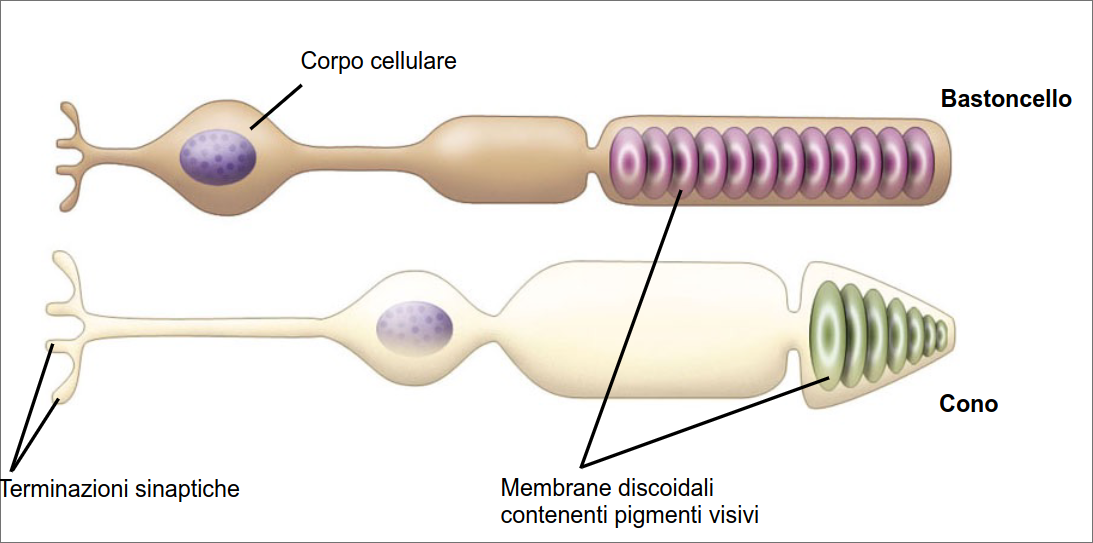
\includegraphics[width=0.8\textwidth]{./resources/rods.png}
    \end{figure}
    \end{center}
\end{snippet}

\plain{Entrando il sodio la membrana depolarizza (dentro diventa più positivo).
    Se la mebrana è depolarizzata, la cellula manda l'impulso.}

\section{Foto bastoncelli al buio e alla luce}

\begin{snippet}{bastoncelli-buio-luce}
    \begin{itemize}
        \item \textbf{Al buio:}
            Il livelli di cGMP sono elevati all'interno del citosol del segmento esterno
            del bastoncello, quindi i canali del sodio localizzati nella membrana del fotorecettore
            si aprono. Il sodio entra perché dentro la differenza di potenziale
            elettrico della cellula è negativo (gradiente elettrochimico).
            Gli ioni sodio entrano nella cellula e determinano una depolarizzazione
            (perché entrano cariche positive, dentro diventa più positivo, potenziale praticamente 0) che viaggia
            dal segmento esterno al terminale del fotorecettore. 
            In risposta alla depolarizzazione, si aprono i canali per il calcio.
            L'ingresso del calcio attiva un processo di esocitosi che porta al rilascio del neurotrasmettitore.
            Il neurotrasmettitore agisce sulle cellule bipolari, generando dei potenziali graduati (le blocca non facendole scaricare)
        \item \textbf{Alla luce:}
            Se c'è luce il pigmento cambia forma. I livelli di cGMP nel citosol del segmento esterno diminuiscono, quindi i canali del sodio si chiudono.
            Il minore ingresso di sodio iperpolarizza la cellula (potenziale negativo all'interno),
            a causa dell'uscita del potassio.
            L'iperpolarizzazione provoca la chiusura dei canali del calcio nel segmento interno,
            quindi viene rilasciato meno neurotrasmettitore dal terminale del fotorecettore.
            La cellula bipolare quindi non riceve nessun segnale, è attiva e quindi scarica
            e di conseguenza anche la gangliare.
    \end{itemize}
\end{snippet}

\section{Difetti della vista}

\begin{snippetdefinition}{miopia-definition}{Miopia}
    Le persone miopi non riescono a mettere bene a fuoco gli oggetti lontani. Il bulbo oculare di
    un individuo miope è più lungo rispetto al normale e il cristallino non può appiattirsi
    abbastanza per compensare. Dunque, gli oggetti vengono messi a fuoco davanti alla retina
    e non direttamente su di essa.
\end{snippetdefinition}

% foto miopia

\begin{snippetdefinition}{ipermetropia-definition}{Ipermetropia}
    Il bulbo oculare è più corto rispetto alla norma e di conseguenza il cristallino mette a fuoco
    le immagini dietro alla retina.
\end{snippetdefinition}

\begin{snippetdefinition}{presbiopia-definition}{Presbiopia}
    Progressiva incapacità dell'occhio di mettere a fuoco gli oggetti vicini, dovuta alla minore
    elasticità del cristallino
\end{snippetdefinition}

\begin{snippetdefinition}{astigmatismo-definition}{Astigmatismo}
    Consiste in uno sfocamento della visione causato da una deformazione del cristallino o della
    cornea che fa convergere in modo non uniforme i raggi di luce, senza focalizzarli su un
    punto unico della retina.
\end{snippetdefinition}

\end{document}